\documentclass[../../Paper.tex]{subfiles}
    
\begin{document}

\subsection*{Data and composition}
\begin{wrapfigure}{r}{0.38\textwidth} 
\centering
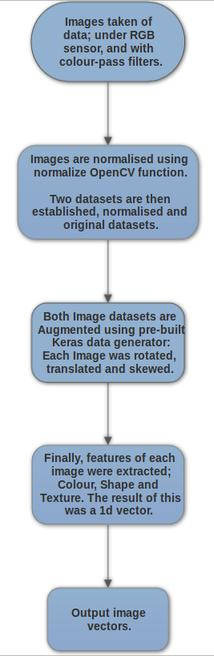
\includegraphics[width=0.33\textwidth, scale = 0.2]{flow_chart2.jpg} 
\caption{Outline of the workflow from raw images to final datasets.}
\end{wrapfigure}


The data used was collected during 2009 and 2017; the 2009 data was collected by Dr Oliver Windram, and the 2017 data was collected by myself and Chris Adams. 

The 2009 data was collected to look at the effect of \textit{Botrytis cineria} on \textit{Arabodopsis thaliana}; the data was collected over a period of 72 hours, allowing us to look at the effect of duration of infection. The time periods for this dataset were 10hpi (hours post infection), 18hpi, 26hpi, 34hpi, 42hpi, 48hpi, 72hpi and non-infected/ control. Images in this dataset were taken under a RGB sensor only. 

The 2017 data was collected to look at the effect of multiple stressors on tomato leaves; a combination of drought stress, Nitrogen deficiency, and \textit{Botrytis cineria} were applied (see Table 1 each treatment type) and left for 42 hours, after which several images were taken, including a RGB image and a range of images under color-pass filters (appendix table 1).

Both datasets were then cropped to contain individual leaf images; once this was done each individual image was processed, as laid out in Figure 3, ready for image classification. 


\subsubsection*{Colour-pass filters}

Part of this papers aim was to ascertain whether colour-pass filters bring out more visual data than just RGB images alone; to test this, three multi-stress datasets were created, with increasing numbers of colour-pass filters used in each. The colour-pass filters were held over a normal RGB sensor camera (Figure 3).

The three datasets consisted of a RGB image dataset (dataset 1), a RGB, purple and magenta image dataset (dataset 2), and a dataset consisting of RGB images and all color-pass filters (dataset 3). The colour-pass filter colours used are noted in Table 1 in the Appendices.

The duration infection dataset did not contain additional filters; only one dataset (dataset 4) was created, containing RGB images.

\subsubsection*{Image Normalisation}

In order to allow for easier comparison between datasets, Dataset 3 was normalised using the normalize function in OpenCV Python (Figure 3). Each image was normalised between absolute black (0) and absolute white (255); the original images were also kept to allow for results comparison. This dataset is referred to as Dataset 3-NORM.

\subsubsection*{Data Augmentation - Reducing over-fitting}

One of the easiest and most common methods of minimising the risks of over-fitting on image data, is to artificially enlarge
the dataset(s) (Figure 3: \cite{simard_best_2003,krizhevsky_imagenet_2012,sladojevic_deep_2016, ubbens_deep_2017}). Another benefit of this approach is that data generation/ augmentation has been noted to improve classifier performance (see:\cite{yaeger_effective_1996}, or \cite{krizhevsky_imagenet_2012}),  by increasing the chance for the classifier to learn appropriate features of each treatment (\cite{sladojevic_deep_2016}). We augmented the dataset using a pre-built data generator in the Keras library (\cite{chollet2015keras}); each image was randomly augmented 20 times using simple  distortions such as translations,  rotations, and  
skewing.

\subsubsection*{Feature extraction}

Prior to training, features of each image dataset (Figure 3: shape, colour, texture) were extracted; this was done as preliminary training was returning poor classification results when trained on the original image dataset. This method of feature extraction is also done to reduce the computational workload, and to further minimise over-fitting. After the features were extracted, each image's data consisted of a 532 x 1 array. 

Test images for each dataset were kept separate from the training datasets; these images consisted of data from the original experiment and from other experiments with the same treatment types.


The final datasets consisted of 3,600 duration infection image vectors; 450 for each stage of infection, and 7,952 multi-stress image vectors; 994 for each treatment. These datasets were split by 80:20 for training/validation of the models. There were also 42 multi-stress test images, and 209 duration infection test images not input into any models; these were used to test the final models for a final accuracy/prediction score.

\begin{table*}[!t]
\centering
\caption{Treatment Types}
\label{my-label}
\begin{tabular}{clllllll}
\cline{3-6}
\multicolumn{1}{l}{}                            & \multicolumn{1}{l|}{}                         & \multicolumn{4}{c|}{Drought}                                                                                                                                                                                              &           &           \\ \cline{3-6}
\multicolumn{1}{l}{}                            & \multicolumn{1}{l|}{}                         & \multicolumn{1}{l|}{Present}                         & \multicolumn{1}{l|}{Absent}                          & \multicolumn{1}{l|}{Present}                         & \multicolumn{1}{l|}{Absent}                          &           &           \\ \cline{1-6}
\multicolumn{1}{|c|}{\multirow{4}{*}{Nitrogen}} & \multicolumn{1}{l|}{\multirow{2}{*}{Present}} & \multicolumn{1}{l|}{\multirow{2}{*}{\textbf{+++}}}   & \multicolumn{1}{l|}{\multirow{2}{*}{\textbf{++ -}}}  & \multicolumn{1}{l|}{\multirow{2}{*}{\textbf{+ - +}}} & \multicolumn{1}{l|}{\multirow{2}{*}{\textbf{+ - -}}} &           &           \\
\multicolumn{1}{|c|}{}                          & \multicolumn{1}{l|}{}                         & \multicolumn{1}{l|}{}                                & \multicolumn{1}{l|}{}                                & \multicolumn{1}{l|}{}                                & \multicolumn{1}{l|}{}                                & \textbf{} & \textbf{} \\ \cline{2-6}
\multicolumn{1}{|c|}{}                          & \multicolumn{1}{l|}{\multirow{2}{*}{Absent}}  & \multicolumn{1}{l|}{\multirow{2}{*}{\textbf{- + +}}} & \multicolumn{1}{l|}{\multirow{2}{*}{\textbf{- + -}}} & \multicolumn{1}{l|}{\multirow{2}{*}{\textbf{- - +}}} & \multicolumn{1}{l|}{\multirow{2}{*}{\textbf{- - -}}} & \textbf{} & \textbf{} \\
\multicolumn{1}{|c|}{}                          & \multicolumn{1}{l|}{}                         & \multicolumn{1}{l|}{}                                & \multicolumn{1}{l|}{}                                & \multicolumn{1}{l|}{}                                & \multicolumn{1}{l|}{}                                & \textbf{} & \textbf{} \\ \cline{1-6}
\multicolumn{1}{l}{}                            & \multicolumn{1}{l|}{}                         & \multicolumn{2}{l|}{Present}                                                                                & \multicolumn{2}{l|}{Absent}                                                                                 &           &           \\ \cline{3-6}
                                                & \multicolumn{1}{l|}{}                         & \multicolumn{4}{c|}{Infection} 
\\ \cline{3-6}                                              
\end{tabular}
\end{table*}


\subsection*{Data modelling}

Image classification problems have utilised various machine learning algorithms in the past, ranging from Linear Regression to Deep CNNs (\cite{naseem_linear_2010,krizhevsky_imagenet_2012,tripathi_recent_2016}).
The two main classification algorithms investigated in this project are Random Forest classifiers, and Convolutional Neural Networks. 


\begin{figure}[!b]
\centering
\begin{subfigure}{.4\textwidth}
  \centering
  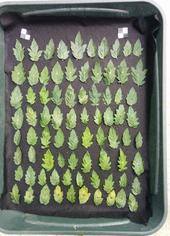
\includegraphics[scale = 0.7]{1_1-2.jpg}
  \caption{Original RGB Image}
  \label{fig:sub1}
\end{subfigure}%
\begin{subfigure}{.4\textwidth}
  \centering
  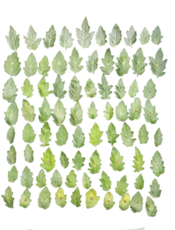
\includegraphics[scale = 0.7]{mask33.png}
  \caption{Masked Image}
  \label{fig:sub2}
\end{subfigure}
\caption{Original RGB Image before and after applying mask}
\label{fig:test}
\end{figure}

Both algorithms have been successfully applied for image classification tasks (\cite{krizhevsky_imagenet_2012,malof_deep_2016}), and are currently being utilised in the field of plant pathology (\cite{awate_fruit_2015, singh_machine_2016}). 


\subsubsection*{Machine Learning}

To get the best classifier comparison, several classifiers were trained on the image data, including Random Forests, K-Nearest-Neighbours and Support Vector Machines.  An ensemble approach was also conducted, consisting of Decision trees, Random Forests and KNNs. Random Forests produced the best results, and so further testing was using RF alone.

Each RF classifier had the same random state, and consisted of 100 trees unless otherwise stated. All RF classifiers then underwent a ten fold cross validation, with accuracy of each classification used as the scoring method. 

The CNN used in this study (Appendix Figure 3) consisted of many layers including several convolutional layers, a dropout layer and, a dense layer. A Relu activation function was used in all convolutional and dense layers; this activation function was used to model nonlinearity in the data, as it
can be computed faster than more traditional functions, such as sigmoid or hyperbolic tangent functions. The dropout layer had a 40\% dropout function, and the learning rate was 15\% unless otherwise stated. The Tensorflow framework (\cite{abadi_tensorflow_2016}) within Python was used to create this CNN.



\subsubsection*{Pixel Intensities}

In order to further validate the predications the classifiers made, and to ensure that there are valid differences between each treatment, pixel intensities were gathered. 

To do this, the background was first masked, so that only the leaves were visible (Figure 4). After this each leaf was labeled in relation to the treatment, and pixel intensities of each treatment leaf were gathered using Python 3.7  (\cite{van_rossum_python_2001}). These Pixel Intensities were then compared using an ANOVA. 


\subsection*{Model comparison}

To compare between classifiers, separate test datasets, consisting of 209 duration images, and 74 treatment images were used to obtain predictions. These predictions consisted of a predicted class and a percentage of certainty, which were also used in comparison analysis. 


\subsection*{Statistical analysis}

All statistical analses were carried out in R version 3.2.3 (\cite{r_core_team_r:_2013}).
ANOVAS (Analysis of Variance) were used to explore variance between treatments within both datasets.





\begin{figure}[!b]
\centering
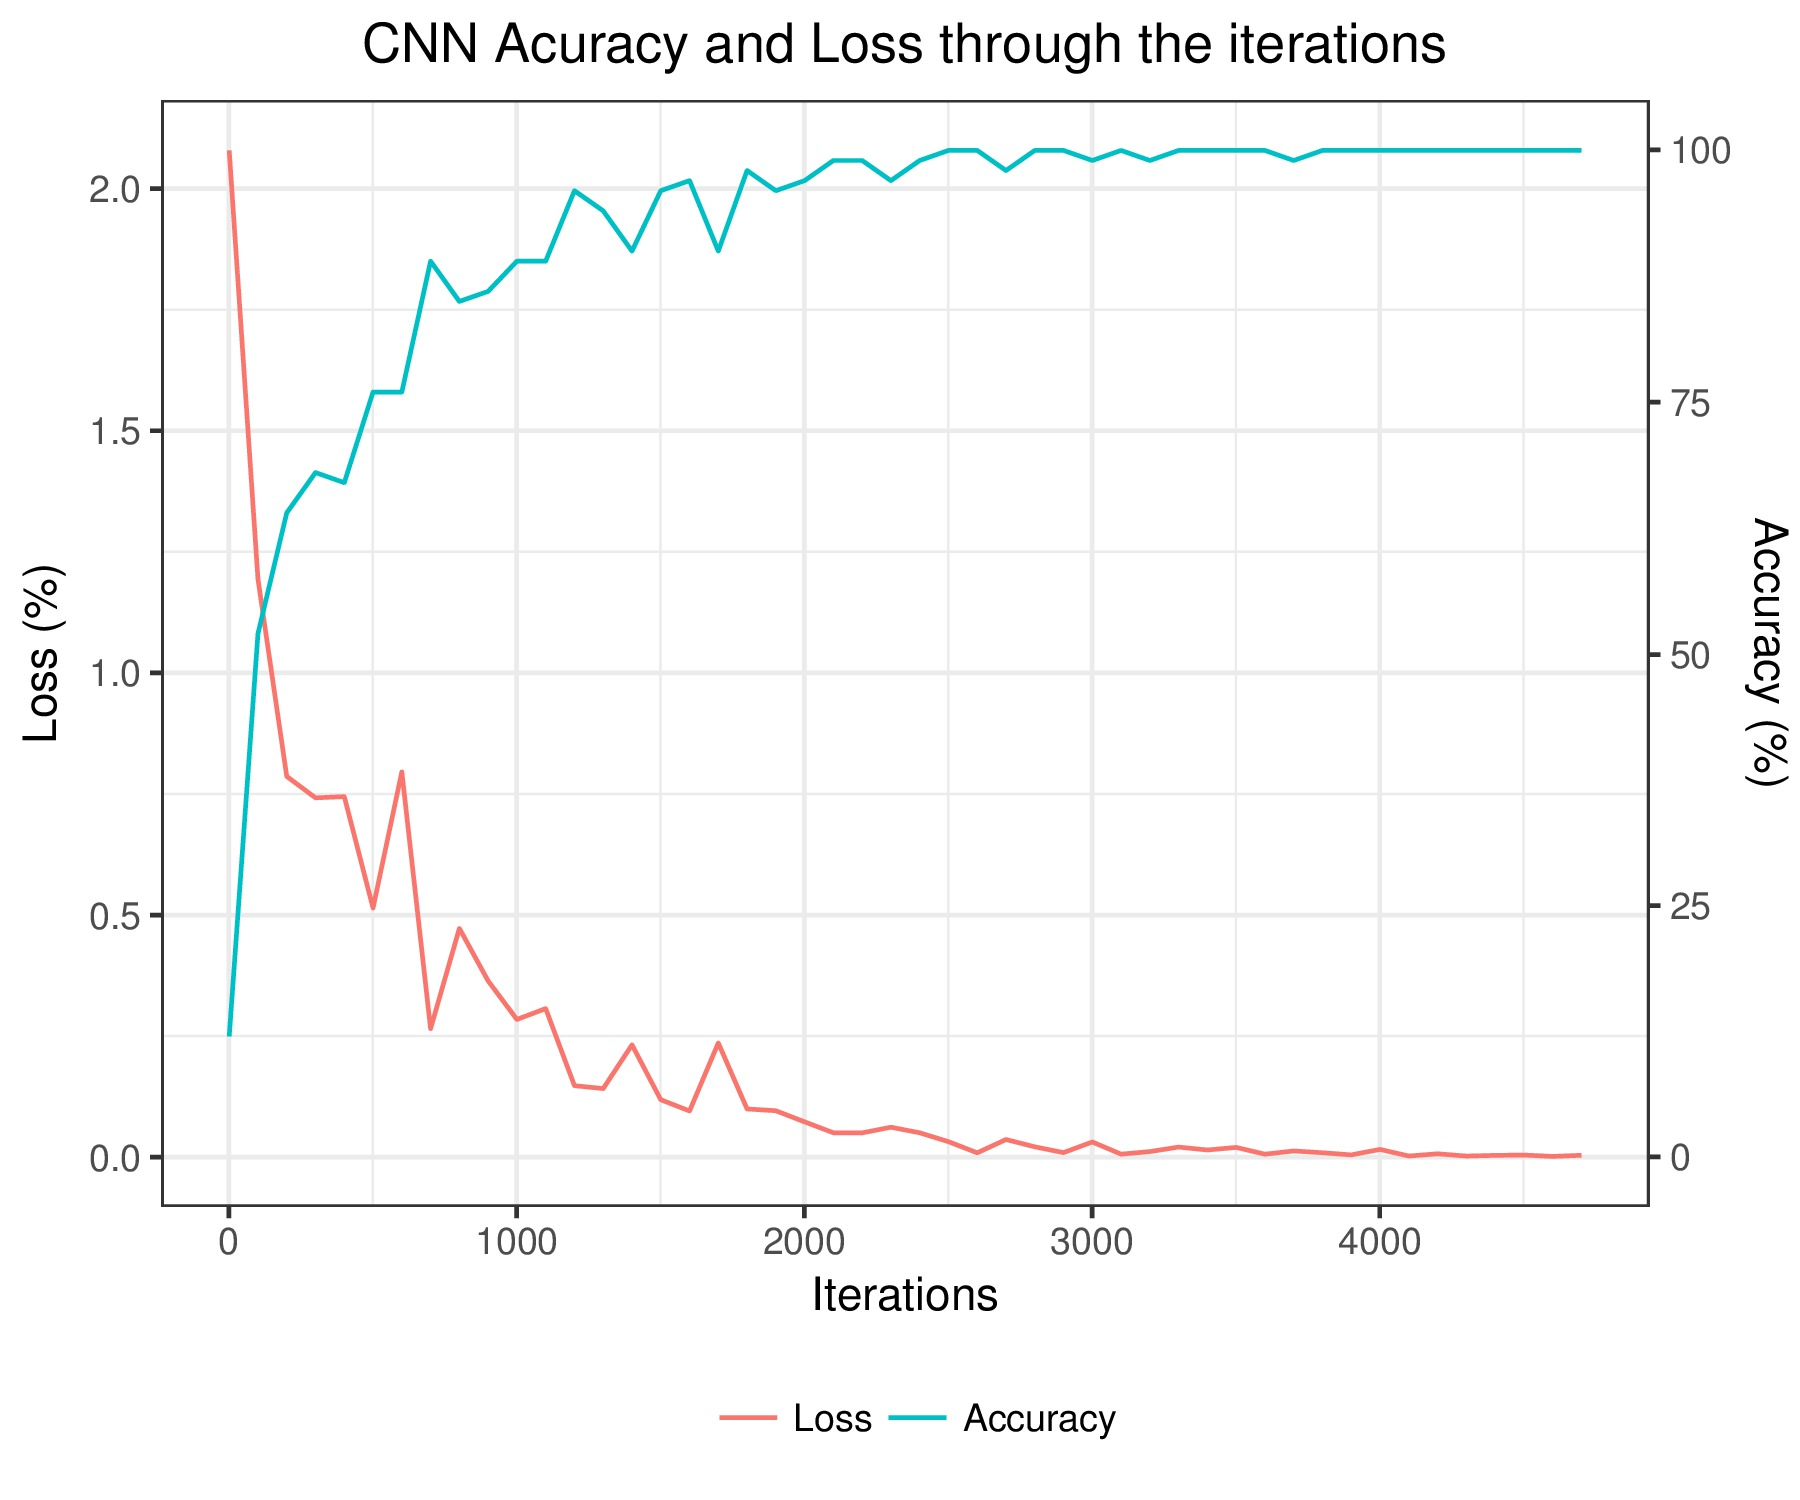
\includegraphics[scale = 0.7]{NN_training.jpg}
\caption{CNN accuracy and loss over 4800 iterations for infection duration classification.}
\end{figure}





\end{document}